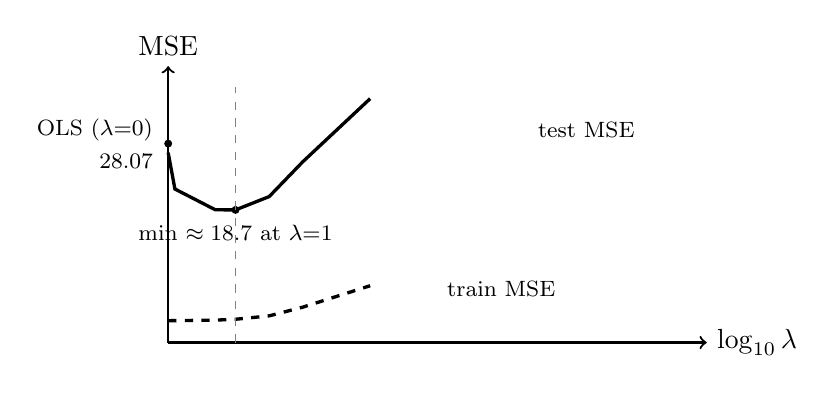
\begin{tikzpicture}[scale=0.9]
\draw[->, thick] (0,0) -- (7.6,0) node[right] {$\log_{10}\lambda$};
\draw[->, thick] (0,0) -- (0,3.9) node[above] {MSE};
% test MSE: OLS 28.07 at lam->0; lams .01 .1 .5 1 3 10 100 -> 26.78 21.66 18.73 18.71 20.59 25.51 34.41
% train MSE: 3.08 3.08 3.09 3.16 3.28 3.76 4.99 8.01
% x=(log10 lam+2)*0.95 ; y=mse*0.1
\draw[very thick] plot coordinates {
  (0,2.678) (0.095,2.166) (0.665,1.873) (0.95,1.871)
  (1.425,2.059) (1.90,2.551) (2.85,3.441)};
\node[font=\footnotesize] at (5.9,3.0) {test MSE};
\draw[very thick, dashed] plot coordinates {
  (0,0.308) (0.095,0.309) (0.665,0.316) (0.95,0.328)
  (1.425,0.376) (1.90,0.499) (2.85,0.801)};
\node[font=\footnotesize] at (4.7,0.75) {train MSE};
% OLS point at left
\fill (0,2.807) circle (1.6pt) node[left=2pt, align=right]
  {\footnotesize OLS ($\lambda{=}0$)\\ \footnotesize 28.07};
\fill (0.95,1.871) circle (1.6pt) node[below=2pt]
  {\footnotesize min $\approx18.7$ at $\lambda{=}1$};
\draw[gray, dashed] (0.95,0) -- (0.95,3.6);
\end{tikzpicture}
